\documentclass[14 pt]{extreport}

\usepackage{extsizes}
\usepackage[utf8]{inputenc} %pour accents
\usepackage[T1]{fontenc}	%pour accents
\usepackage[francais]{babel}%pour langue
%\usepackage[textwidth=18cm,textheight=22cm]{geometry} %mise en page
\usepackage{hyperref}	%URL
\usepackage{listings}	%code
\usepackage{amsmath}
\usepackage{graphicx}
\usepackage{epstopdf}
\usepackage{lipsum}
\usepackage{smile_template}
\usepackage{fancyvrb}
\usepackage[section]{placeins}
\usepackage{float}% If comment this, figure moves to Page 2
\epstopdfsetup{outdir=./}

\usepackage{fancyhdr}

  \lstdefinestyle{ascii-tree}{
    literate={├}{|}1 {─}{--}1 {└}{+}1 
  }

\pagestyle{fancy}
\setlength{\unitlength}{1mm}
\addtolength{\headheight}{1.5\baselineskip}
\renewcommand{\headrulewidth}{0.4pt}
\renewcommand{\footrulewidth}{0.4pt}
\rhead{
%
\includegraphics[width=3cm]{images/Logo_Smile_400.jpg}
}

% Redefine the plain page style
\fancypagestyle{plain}{%
  \fancyhf{}%
  \fancyfoot[C]{\thepage}%
  \renewcommand{\headrulewidth}{0pt}% Line at the header invisible
  \renewcommand{\footrulewidth}{0.4pt}% Line at the footer visible
}

\title{\textbf{Rapport de stage de fin d'études}}
\author{Martin Guilloux}


\begin{document}

\maketitle

\section*{Résumé}
Dans le cadre de ma dernière année d'études à l'INSA Centre-Val-de-Loire, j'ai effectué un stage de six mois, l'aboutissement de trois ans passés à l'institut. J'ai effectué ce stage au sein de l'équipe Outsourcing de l'entreprise Smile, à Montpellier. Smile est une entreprise d'hébergement et de développement de websites/webservices française, s'appuyant pour cela sur le monde de l'Open Source.

Ce stage m'a fait expérimenter plusieurs technologies, notamment liées à l'automatisation et à la virtualisation.

\section*{Remerciements}
Je remercie mon enseignant référent Benjamin NGUYEN, d'avoir encadré le déroulement de mon stage.\\
Merci également à Mathieu BLANC, mon maître de stage, pour sa bonne humeur et ses bons conseils.\\
Je remercie aussi toute l'équipe Outsourcing de Smile Montpellier, pour l'accueil et la bonne ambiance quotidienne : Syben, Daber, Adbig, Cebri, Wibru, Secal, Jocor, Dyfei, Segir, Mohla, Aulem, Flmag, Pamar, Alniz, Niper, Alwie, merci d'avoir été plus que de simple collègues de travail.\\
Merci aussi à tout le reste de l'équipe Smile Outsourcing, avec qui j'ai discuté au quotidien.


\tableofcontents

\chapter*{Summary, keywords}
\section*{Summary}
\lipsum[1]\lipsum[1]
\section*{Keywords}
\lipsum[1]


\chapter*{Glossaire}

\begin{itemize}

\item{\textbf{Automatisation}}: Ensemble de techniques permettant le déroulement autonome d'un système, en interconnectant plusieurs élements de ce système ; Par exemple, la génération d'un fichier pdf et l'envoi de ce fichier par mail, tout ceci sans intervention directe humaine.

\item{\textbf{AS}}: Système Autonome, ensemble de réseaux IP sous le contrôle d'une entité/organisation unique (ex. entreprise, FAI...)

\item{\textbf{container}}: système d'exploitation isolé à l'intérieur d'un autre système, permettant ainsi à un hôte de virtualisation de faire tourner plusieurs systèmes sur une seule machine physique. (ex. de systèmes de conteneurisation : docker, lxc, openVZ)

\item{\textbf{BGP}}: Pour \emph{Border Gateway Protocol} - Protocole d'échange de routes entre différents AS, notamment sur le réseau Internet

\item{\textbf{Orchestration}}: Processus automatique d'organisation, de coordination et de gestion de systèmes informatiques, de middlewares et de services.

\item{\textbf{Datacenter}}: Site physique regroupant un grand nombre d'équipements de système d'information (Serveurs, core routeurs, switchs, firewalls...)

\item{\textbf{Ansible}}: Plate-forme logicielle d'automatisation Open Source en python, détenue par Red Hat. Ansible s'appuie sur ssh et utilise un modèle agentless ne nécessitant pas d'installer un client sur chaque noeud géré.

\item{\textbf{Puppet}}: Une autre plate-forme logicielle d'automatisation Open Source, écrite en ruby, développée par Puppetlabs. Puppet est basé sur un modèle master-slaves, il est nécessaire d'installer un agent sur chaque noeud, qui exécute le catalogue d'instruction envoyé par le puppetmaster.

\item{\textbf{ENC}}: Pour External Node Classifier - Programme externe à Puppet interrogé par le puppetmaster, chargé de gérer pour chaque noeud la liste des classes et des paramètres qui lui sont attribués. (Par exemple, l'outil puppet-dashboard, en plus de fournir une interface web de résumé des puppet run, offre aussi la possibilité d'être utilisé comme ENC)

\item{\textbf{Rôle Ansible}}: ensemble de fichiers d'intructions écrites en yaml permettant à Ansible d'effectuer ces instructions sur les noeuds qu'il gère. Ce rôle peut être invoqué depuis n'importe quel \emph{playbook} Ansible. Un équivalent en programmation serait une bibliothèque C ou un module Python, qu'on peut appeler depuis n'importe quel programme

\item{\textbf{Playbook}}: Ensemble d'instructions exécutées sur un certain nombre de noeuds par Ansible, écrit en yaml. Il comprend notamment la liste des noeuds sur lesquels s'exécuter, les permissions requises, ainsi qu'une liste de rôles Ansible et des variables.

\item{\textbf{Manifest Puppet}}: Code écrit en langage Puppet s'exécutant sur les puppet agents. L'équivalent d'un rôle Ansible.

\end{itemize}

\chapter{Introduction}

\section{Cadre et objectifs du stage}

\subsection{Le stage}L'intitulé de mon stage, "Industrialisation des méthodes de déploiement de plates-formes d'hébergement Internet", suggère la mise en place et la convergence de plusieurs outils pour améliorer à la fois les temps de traitement et la qualité des déploiements de plates-formes d'hébergement. Dans cette optique le travail a été décomposé en plusieurs phases, la première consistant à comprendre le fonctionnement du système existant, l'architecture réseau des serveurs de production de Smile, la base technique en place, ainsi que le périmètre impacté par l'ensemble des modifications à apporter. Il a fallu ensuite mettre en place ou améliorer des solutions dans un souci d'amélioration continue, tout en maintenant et en adaptant l'existant de manière à permettre la cohabitation entre les systèmes de production d'aujourd'hui et de demain.

Avant de parler plus en détail des tâches que j'ai été amené à accomplir, une présentation de l'entreprise qui m'a accueilli pendant ces six mois.

\subsection{Présentation de Smile}
\lipsum
Historique

Description offre commerciale

\chapter{Découverte du réseau de production et de la base technique}

A mon arrivée chez Smile, j'ai commencé par effectuer un tour des technologies utilisées, ainsi que du réseau de production sur lequel j'allais être appelé à travailler. J'ai ainsi pu dégager les points sur lesquels il faudrait agir et isoler les problématiques des différents composants du système de production.

En parallèle je me suis documenté sur les technologies et les outils que j'allais utiliser tout au long de mon stage, notamment Puppet et Ansible.

\section{Présentation du réseau de production}

Les serveurs de production de Smile sont répartis sur trois \emph{datacenters} : Deux dans les environs de Paris (Equinix PA3 à Saint-Denis et Iliad à Vitry-sur-Seine), et un à Lyon (Datacenter SFR à Venissieux) rajouté récemment suite au rachat par Smile de OpenWide Outsourcing (OWO). La convergence avec OWO étant en cours, j'ai été amené à travailler uniquement sur des serveurs présent dans les DC de Paris. Dans chacun de ces deux DC se trouve un Core Router Cisco (cr1 et cr2) ainsi que deux firewalls (fw3,4 et fw5,6), à savoir des serveurs dell sous openBSD. Cette répartition entre plusieurs DC fait suite à la volonté de Smile de mettre en place un Plan de Reprise d'Activité (PRA) incluant des \emph{datacenters} distants de plus de trente kilomètres.

Les core routers et les firewalls sont interconnectés entre les deux sites par fibre optique et administrés sur un vlan spécifique, de même que les serveurs derrière les firewalls (sur un autre vlan).

\begin{figure}[htp]
\centering
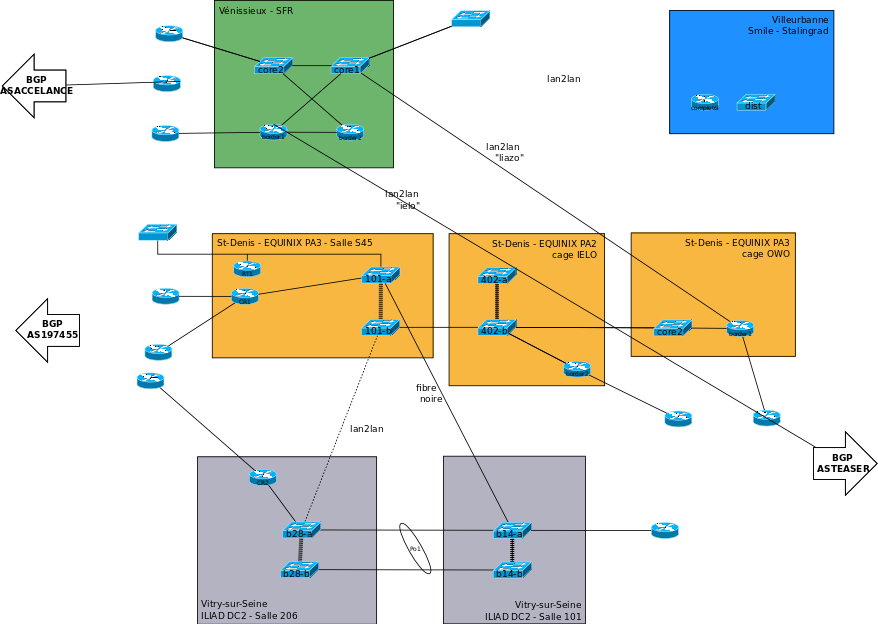
\includegraphics[scale=0.4]{reseau_backbone.png}
\caption{Schéma récapitulatif du réseau backbone de Smile}
\label{}
\end{figure}
%TODO insérer schéma réseau Smile
\section{Le socle technique de la production}

Je vais ici présenter un résumé des technologies utilisées par le système de production chez Smile, en deux parties : les technologies de virtualisation et le système de monitoring, et enfin le système d'orchestration en place, utilisant puppet dont je présenterai rapidement le fonctionnement.
\subsection{Technologies de virtualisation et de monitoring}
\paragraph{Virtualisation :}Les sites hébergés par Smile le sont dans des containers openVZ, avec pour hôtes de virtualisation des serveurs physiques tournant sous CentOS. Les VM sont nommées en fonction du client et du rôle qu'elles jouent dans le système du site web (par exemple youboost-postgresdb1.priv.smile-hosting.fr pour une VM de base de donnée de youboost, ou gifi-pp.priv.smile-hosting.fr pour une VM de pré-production). Les hôtes de virtualisation quand à eux sont nommés en fonction du client dans le cas d'un serveur dédié (ex. gifi-host3.vpn.ti.smile.fr) ou shared-host dans le cas de serveur mutualisé (les serveurs mutualisés sont cependant appelés à migrer vers un cluster utilisant KVM).

Le déploiement de nouveaux hôtes de virtualisation se faisait en PXE, puis sa configuration se faisait à la main ou par le biais de scripts shell.

%TODO schéma openVZ

\paragraph{Monitoring :}Le système de production possède plusieurs facettes qui nécessitent d'être monitorées : Il faut surveiller le bon fonctionnement des backups (basés sur bacula et des scripts utilisant rsync), mais aussi la charge réseau entre les différents datacenters (et potentiellement répartir la charge entre les deux DC), et enfin l'état de tous les serveurs de production.

Pour cela plusieurs outils sont utilisés : Pour les backups un outil interne remonte les informations sur l'état des backups via une page web, tandis que la charge réseau est surveillée via snmp et graphée avec \emph{Cacti}. Pour monitorer l'état des serveurs, enfin, Smile utilise un fork de \emph{Nagios} écrit en python : \emph{Shinken} ainsi qu'une interface web pour afficher ses données, \emph{Thruk}. L'équipe de production utilise également un outil interne de monitoring, \emph{suri5} pour monitorer les sites clients et pour remonter des alertes. Tous ces logiciels sont bien sûr Open Source (un mouvement fortement ancré dans le fonctionnement de Smile, même si cette tendance semble évoluer ces derniers temps).

\subsection{Présentation du système d'orchestration}

Le système d'orchestration à mon arrivée était entièrement basé sur Puppet, un système d'automatisation et d'orchestration Open Source édité par Puppetlabs et écrit en Ruby que je vais rapidement présenter.

Puppet est basé sur un système \textbf{agent-serveur}, c'est à dire que sur chaque noeud géré par puppet il faut installer un \textbf{agent} puppet (présent dans le paquet puppet de base) et le configurer pour se connecter au puppetmaster, le serveur gérant chaque noeud. Un service lance l'agent toutes les heures en temps normal, mais sur une architecture telle que celle de Smile, les temps de traitement excèdent cette durée, c'est donc un \emph{cron} qui lance une \emph{puppet run} deux fois par jour pour éviter la surcharge du puppetmaster (cette cron est générée elle-même lors de chaque run puppet, comme je l'expliquerai un peu plus loin)

Lors de cette run, l'agent se connecte au puppetmaster de manière sécurisée (la suite puppet inclut une autorité de certification qui permet d'ouvrir des connexions sécurisées par SSL). Une fois cette étape d'authentification effectuée, l'agent rassemble des informations sur le système sur lequel il s'exécute. Il envoie ensuite ces informations au puppetmaster, qui s'en sert pour génerer une série d'instructions qui sont renvoyées à l'agent, ce dernier les exécutant et renvoyant en fin de run un résumé de l'état de sortie de chaque instructions, permettant de constater les erreurs de traitement ou les fichiers modifiés (par exemple).

Ci-après, un schéma récapitulatif des interractions au cours d'une puppetrun. On peut constater que la run a lieu en trois temps, d'abord une connexion agent $\rightarrow$ master, pendant laquelle le noeud envoie ses informations (des \emph{facts}), puis master $\rightarrow$ agent, durant laquelle le puppetmaster envoie le catalog au noeud, et enfin une dernière connexion agent $\rightarrow$ master pour le reporting.

\begin{figure}[H]
\centering
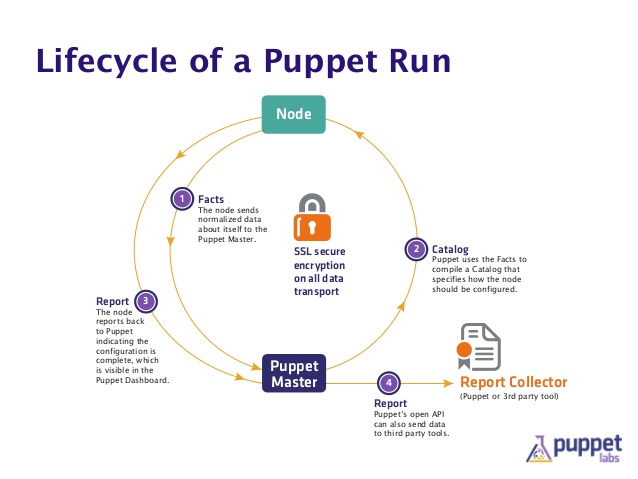
\includegraphics[scale=0.70]{puppetrun.jpg}
\caption{schéma volé éhontément dans une keynote puppetlabs}
\label{}
\end{figure}

Avant de poursuivre, il est nécessaire d'introduire un peu de vocabulaire spécifique à puppet.

Pour savoir quelles instructions exécuter sur un noeud, puppet utilise un système de \emph{manifests} écrits en "langage puppet", un langage à la syntaxe assez spécifique (voir un exemple de manifest puppet en annexe 1) mais relativement simple à comprendre, ainsi qu'un système de \emph{templating} basé sur \emph{erb} (Embedded RuBy) pour pousser des fichiers de configuration sur les noeuds. Ces manifests se divisent en classes, elles-mêmes divisées en ressources. Avec puppet, tout est ressource.\footnote{Paracelse ajouterait que "rien n'est ressource, c'est la dose qui fait la ressource."} Une ressource est en effet l'unité fondamentale d'instruction en puppet. Par exemple, déclarer une ressource de type \emph{file} dans un manifest donnera l'instruction de transférer un fichier (depuis le puppetmaster ou n'importe quelle URI, ou encore d'après un template), tandis qu'une ressource \emph{exec} permettra d'exécuter une commande directement dans le shell de la machine distante (encore une fois, voir en annexe 1 pour un exemple de code puppet)

\begin{itemize}
	\item Une classe est une suite de déclarations de ressources, qui peut être incluse dans un manifest (et ainsi éviter de retaper le même code plusieurs fois) avec des paramètres spécifiés lors de l'écriture de la classe. Par exemple une classe xmpp::client pourrait recevoir un paramètre pour savoir à quel serveur xmpp le client doit se connecter, afin de gérer les fichiers de configuration xmpp correctement.
	\item Un manifest, quant à lui, est un ensemble de ressources et d'inclusions de classes, en somme un fichier puppet générique.
	\item Un module Puppet est un ensemble de manifests, de fichiers, de répertoires et de templates rassemblés dans un but de portabilité. Il peut aussi contenir des fichiers ruby exécutés sur l'hôte distant pour générer des \emph{facts} supplémentaires.
	\item Un catalog Puppet est un ensemble d'instructions envoyées par le puppetmaster à un noeud après les avoir "compilées".
\end{itemize}

Ci-dessous, l'arborescence typique d'un module puppet.
\newpage
\begin{Verbatim}[fontsize=\tiny]
magui@puppetmaster-v4:~/puppet/modules/puppetnode (bacula-lxc)$ tree
.
+-- files
|   +-- etc
|   |   +-- profile-lenny.default
|   |   \-- profile-lenny.puppet
|   +-- etc-default-puppet
|   +-- nrpe
|   |   \-- check_puppet.sh
|   +-- puppet.conf.preprod
|   +-- puppet.conf.prod
|   +-- puppet-cron-cleaning-tasks
|   +-- puppetlabs-pinning
|   \-- tools
|       \-- facter
|           \-- util-ip-patched.rb
+-- lib
|   \-- facter
|       +-- all_vzchildren_fqdn.rb
|       +-- interfaces_with_link.rb
|       +-- lamp_stack_versions.rb
|       +-- majdistrelease.rb
|       +-- pam_bash_users.rb
|       +-- puppetrun_cronjob.rb
|       +-- resolv_domain.rb
|       \-- utc_offset_hours.rb
+-- manifests
|   +-- announce
|   |   \-- register.pp
|   +-- announce.pp
|   +-- collector.pp
|   +-- config.pp
|   +-- cron.pp
|   +-- init.pp
|   +-- nrpe.pp
|   +-- puppetscript.pp
|   +-- service.pp
|   \-- tools
|       +-- all.pp
|       +-- facter.pp
|       +-- lsbrelease.pp
|       +-- puppetlabs_repository.pp
|       \-- ruby.pp
+-- metadata.json
\-- templates
    +-- collector-cron.part.erb
    +-- cron-smile-puppet.erb
    \-- puppet.conf.erb

\end{Verbatim}


Lors d'une run puppet, le puppet-dashboard de Smile fait office d'ENC\footnote{voir le glossaire} pour déterminer quelles classes appliquer à chaque noeud. Il lit ensuite les manifests et les adapte au noeud en renseignant les variables (on pourrait faire une analogie avec l'étape des directives de préprocesseur dans une compilation), avant d'envoyer un \emph{catalog} au noeud qui les exécute.

Une autre composante essentielle du système d'orchestration de Smile est l'utilisation de \emph{hiera}. Il s'agit d'un système permettant de stocker des variables en dehors des manifests dans des fichiers yaml. Dans le cas de Smile hiera est utilisé pour stocker les variables spécifiques à chaque serveur, permettant de gérer les spécificités de chaque machine de manière centralisée.

\chapter{Les évolutions apportées}

\lipsum
\lipsum
\lipsum

\chapter{Autres missions}
\lipsum

\chapter{Conclusion, bilan}
\lipsum

\end{document}
